\begin{problem}{三星珠}{三星珠.in}{三星珠.out}{1 second}


这是一道有香味的题!Mr Zhou在某宝上买了好多的美味巧克力,一共$N$块。但是为了让USSTSIW的小朋友们帮他一起分担热量,因此他决定把这$N$块巧克力切割成$M$份,分给$M$个同学,但是为了保证公正公平,分给这$M$个同学的巧克力长度必须相同,现在Mr Zhou想要知道怎么样切割这些巧克力,使得这$M$个同学所得的巧克力最长(假设$N$种巧克力的长度可能各不相同),并计算出巧克力的最佳切割长度$L_{max}$等于多少,结果保留1位小数。
\begin{center}
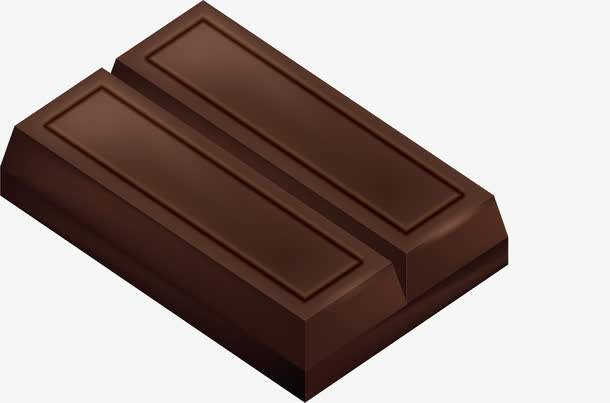
\includegraphics[width=0.5\textwidth]{pics/C.jpg}
\end{center}
\InputFile

第一行输入两个正整数$N\ (1\le N\le 10000)$和$M\ (1\le M\le 1000)$;

接下来输入$N$个数$a_1,a_2,\cdots,a_N$表示每根巧克力的长度$(1\le a_i\le 10000)$。

\OutputFile

输出巧克力的最佳切割长度,结果保留1位小数(无需四舍五入,如计算得到2.26,则输出2.2)。

\Examples

\begin{example}
\exmp{
5 12
5.89 2.36 1.0 8.56 9.13
}{
2.0
}%
\end{example}
\\
\end{problem}
